\section{论证的分析}

\begin{logicbox}[title=引言]
\textit{论证分析是逻辑学中至关重要的技能,通过系统的分析方法可以清晰地展现复杂论证的结构和逻辑关系。}
\end{logicbox}

在现实中,论证的复杂程度差异很大。\logicemph{简单论证}可能只包含一个前提和一个结论,而\logicemph{复杂论证}则可能包含多个前提,这些前提以不同方式为结论提供支持。此外,论证中命题的数量、排列顺序以及相互关系也会呈现出多样化的特征。

为了准确理解和评估各种论证,我们需要掌握系统的\logicterm{论证分析技法},这些方法能够帮助我们清晰地揭示前提与结论之间的逻辑关联,从而更好地把握论证的内在结构。

\begin{theorembox}[title=两种主要分析方法]
论证分析主要有两种系统性方法:
\begin{itemize}
  \item \logicterm{解析法}(paraphrase):用清晰的语言和逻辑顺序重新表述论证中的各个命题,明确标识前提和结论
  \item \logicterm{图示法}(diagram):运用二维空间关系图直观地展示论证的逻辑结构和命题间的支持关系
\end{itemize}

这两种方法各有优势,可以根据论证的具体特点和分析需要选择最适合的方法,有时也可以结合使用。
\end{theorembox}

\subsection{解析法}

\logicterm{解析法}的核心是将原始论证重新组织,用清晰、简洁的语言明确列出各个前提和结论。让我们通过一个具体例子来说明:

\begin{examplebox}[title=原始论证]
现代鸟类并非从直立行走的兽脚类恐龙(包括霸王龙)进化而来,有三个主要理由。首先,大多数类鸟兽脚类恐龙化石发源时间比初始鸟类遗留的化石晚七千五百万年。……其次,鸟的祖先必定已适宜飞行,而兽脚类恐龙并不适宜飞行。第三个理由在于……兽脚类恐龙都有锯状牙齿,而鸟类没有锯状牙齿。${}^{[10]}$
\end{examplebox}

通过解析法,我们可以将这个论证的逻辑结构清晰地展现出来:

\begin{examplebox}[title=解析后的论证结构]
\logicemph{前提}:
\begin{enumerate}
  \item 类鸟兽脚类恐龙化石比初始鸟类遗留的化石发源时间要晚得多
  \item 鸟的祖先必定已适宜飞行,但兽脚类恐龙不适宜飞行
  \item 兽脚类恐龙都有锯状牙齿,而鸟类没有锯状牙齿
\end{enumerate}

\logicemph{结论}:现代鸟类并非从直立行走的兽脚类恐龙进化而来
\end{examplebox}

\logicemph{解析法的重要价值}在于它能够揭示论证中的\logicterm{隐含假设}和\logicterm{未明述前提}。通过系统的分析,我们可以发现原始表述中被默认但未明确说出的逻辑环节。

\begin{examplebox}[title=揭示隐含前提的例子]
大数学家哈代曾说:
\begin{quotation}
阿基米得将被永远记住而埃斯库罗斯会被遗忘,因为一种语言会消亡而数学理念不会消亡。${}^{[11]}$
\end{quotation}

通过解析法,我们可以揭示这个论证的完整逻辑结构:

\logicemph{第一个子论证}:
\begin{enumerate}
  \item 一种语言会消亡
  \item 埃斯库罗斯的伟大剧作使用一种语言
  \item 因此,埃斯库罗斯的成果终究会消亡
\end{enumerate}

\logicemph{第二个子论证}:
\begin{enumerate}
  \item 数学理念不会消亡
  \item 阿基米得的伟大工作使用数学理念
  \item 因此,阿基米得的成果不会消亡
\end{enumerate}

\logicemph{总结论}:阿基米得将被永远记住而埃斯库罗斯将被遗忘
\end{examplebox}

这种深入分析揭示了哈代这句话实际上包含了一个复杂的论证链,其中包含了若干可能存在争议的隐含前提。

\subsection{图示法}

\logicterm{图示法}是另一种强有力的论证分析工具,它通过视觉化的方式直观地展现论证的逻辑结构。图示法的基本步骤包括:

\begin{theorembox}[title=图示法的操作步骤]
\begin{enumerate}
  \item 为论证中的每个命题分配一个编号,并用圆圈标示
  \item 用箭头表示前提与结论之间的支持关系
  \item 通过图形布局直观展现论证的逻辑结构
\end{enumerate}
\end{theorembox}

图示法的优势在于它能够简洁地展现复杂的逻辑关系,避免重复叙述命题内容。让我们通过一个例子来说明:

\begin{examplebox}[title=图示法应用实例]
\begin{quotation}
(1)与许多人的认识相反,HIV检测呈阳性并不必定是死亡判决。一方面,(2)从(艾滋病病毒)抗体生发到出现临床症状平均将近十年时间;另一方面,(3)许多研究报告显示,相当数量的检测呈阳性者从未发展为艾滋病患者。${}^{[12]}$
\end{quotation}

使用图示法,我们可以清晰地展现这个论证的结构:
\end{examplebox}

\begin{center}
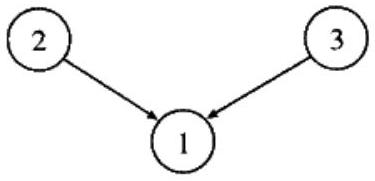
\includegraphics[width=\textwidth]{images/2025_05_15_6a28331d5e7c993ad07ag-030.jpg}
\end{center}

\logicwarn{图示法的适用性}:对于简单直接的论证,图示法可能显得过于复杂;但对于结构复杂的论证,图示法能够在二维平面上直观地展现逻辑关系,具有独特的优势。${}^{[13]}$

\begin{theorembox}[title=图示法的布局原则]
\begin{itemize}
  \item \logicterm{结论}通常置于图示的下方
  \item \logicterm{前提}置于结论的上方
  \item 同层级的前提在图中水平排列
  \item 箭头方向从前提指向结论
\end{itemize}
\end{theorembox}

图示法的一个重要优势是能够清晰地展现\logicemph{前提支持结论的不同方式}。在上述HIV检测的例子中,前提(2)和(3)都\logicemph{独立地}支持结论(1)。这意味着:
\begin{itemize}
  \item 每个前提单独就能为结论提供一定的支持
  \item 即使缺少其中一个前提,另一个前提仍能支持结论
  \item 这种\logicterm{分立性支持}在图示中通过分别的箭头清晰地表现出来
\end{itemize}

与分立性支持不同,有些论证中的前提必须\logicemph{联合起来}才能有效支持结论。这种情况下,单个前提无法独立提供充分的支持。

\begin{examplebox}[title=联合支持的例子]
\begin{quotation}
(1) 我们应该允许安乐死,(2) 如果这样做是最适当地维护所有当事人的利益的话。(3) 而有时候安乐死确实是最适当地维护所有当事人的利益。(4) 因此我们有时候应该允许安乐死。${}^{[14]}$
\end{quotation}

在这个论证中,前提(2)和(3)必须联合起来才能支持结论(4):
\end{examplebox}

\begin{center}
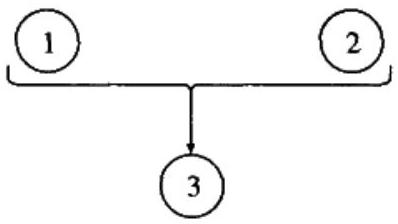
\includegraphics[width=\textwidth]{images/2025_05_15_6a28331d5e7c993ad07ag-031(1).jpg}
\end{center}

\begin{theorembox}[title=联合支持的特征]
在图示中,我们用\logicemph{托架线}连接需要联合支持的前提,这表明:
\begin{itemize}
  \item 单个前提无法独立支持结论
  \item 只有当所有相关前提都为真时,结论才能得到支持
  \item 缺少任何一个前提,整个论证就失去了说服力
\end{itemize}

在上述例子中:
\begin{itemize}
  \item 仅有原则(2)而无具体情况(3),结论无法成立
  \item 仅有具体情况(3)而无指导原则(2),结论同样无法成立
  \item 只有两个前提同时为真,结论才能得到有效支持
\end{itemize}
\end{theorembox}

\subsection{复杂论证的分析}

当论证结构变得复杂时,图示法的优势就更加明显。它能够清晰地展现那些用文字描述可能显得混乱的逻辑关系。

\begin{examplebox}[title=混合支持模式的复杂论证]
\begin{displayquote}
(1)沙漠高地是天文观测的良好场所。(2)其高度使得它们坐落于大气层之中,使得星光不用穿越整个大气层而到达望远镜。(3)沙漠的干燥度也使之相对较少受云雾干扰。(4)云雾对天空的遮蔽会使许多天文观测归于无用。${}^{[15]}$
\end{displayquote}

\logicemph{结构分析}:
\begin{itemize}
  \item 命题(1)是论证的\logicterm{结论}
  \item 命题(2)\logicemph{独立支持}结论——高度优势本身就足以说明沙漠高地适合天文观测
  \item 命题(3)和(4)\logicemph{联合支持}结论——必须结合起来才能构成完整的论证链
\end{itemize}

这个论证展现了\logicwarn{混合支持模式}:既有独立支持,又有联合支持。
\end{examplebox}

\begin{center}
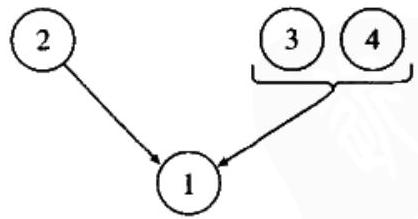
\includegraphics[width=\textwidth]{images/2025_05_15_6a28331d5e7c993ad07ag-031.jpg}
\end{center}

\logicwarn{方法选择的考虑}:虽然图示法在展现复杂结构方面很有优势,但在某些情况下,解析法可能更为有效。特别是当论证包含\logicemph{隐含前提}时,解析法能够更直接地处理这些未明述的假设。

\begin{examplebox}[title=处理隐含前提的例子]
\begin{quotation}
只有当我能够做出其他选择时,我对我的行为才负有道德责任。因为一个人若无力避免某行为,就不应被认为对该行为负有道德责任。${}^{[16]}$
\end{quotation}

这个论证在表面上看起来是完整的,但实际上缺少一个关键的连接环节。
\end{examplebox}

\begin{theorembox}[title=解析法揭示隐含前提]
通过解析法,我们可以清晰地展现完整的论证结构:

\logicemph{明述前提}:
\begin{enumerate}
  \item 一个人若无力避免某行为,就不应被认为对该行为负有道德责任
\end{enumerate}

\logicemph{隐含前提}:
\begin{enumerate}
  \setcounter{enumi}{1}
  \item 只有当我能够做出其他选择时,我当下的行为才是我有能力避免的
\end{enumerate}

\logicemph{结论}:
只有当我能够做出其他选择时,我对我的行为才负有道德责任

\logicwarn{优势}:解析法能够直接列出隐含前提,而图示法则需要用特殊符号(如虚线圆圈)来标示补充的前提。
\end{theorembox}

\subsection{多重复合论证}

当文本包含多个相互关联的论证时,图示法能够清晰地展现这些论证之间的复杂关系。这种情况在政治文献、学术论文等复杂文本中经常出现。

\begin{examplebox}[title=多重论证的实例]
下面是马克思给恩格斯信件中的一段话:
\begin{displayquote}
(1)加速英国的社会革命就是国际工人协会的最重要的目标。(2)而加速这一革命的唯一办法就是使爱尔兰独立。因此,(3)国际的任务就是到处把英国和爱尔兰的冲突提到首要地位,(4)到处都公开站在爱尔兰方面。${}^{[17]}$
\end{displayquote}
\end{examplebox}

\begin{theorembox}[title=多重论证的识别原则]
\logicemph{论证数量的判断标准}:
\begin{itemize}
  \item 一段文字中论证的数目通常等于其中结论的数目
  \item 每个结论对应一个独立的论证
  \item 不同论证可能共享相同的前提
\end{itemize}

在上述例子中:
\begin{itemize}
  \item 有两个结论:(3)和(4)
  \item 因此包含两个论证
  \item 两个论证共享相同的前提:(1)和(2)
\end{itemize}
\end{theorembox}

\begin{center}
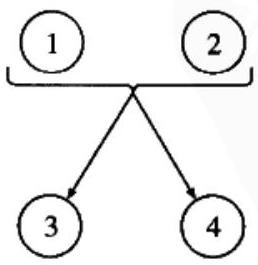
\includegraphics[width=\textwidth]{images/2025_05_15_6a28331d5e7c993ad07ag-032.jpg}
\end{center}

有时,含有两个结论从而有两个论证的一段话,却只含有一个前提。例如:

\begin{quotation}
年纪较大的妇女更难以抵制工作中的性骚扰和离开施暴的丈夫,因为年龄的偏见使她们不容易找到其他保护自己的方式。${}^{[18]}$
\end{quotation}

其中唯一的前提是年纪较大的妇女不容易找到保护自己的方式。该前提支持两个结论:年纪较大的妇女难以抵制工作中的性骚扰,以及她们(对已婚妇女而言)难以离开施暴的丈夫。我们通常用"\logicemph{单独论证}"一词指谓只有一个结论的论证,而不管有多少用以支持它的前提。

\subsection{论证中的命题次序}

当一段话中出现两个或更多论证,或一个论证中有两个或更多前提时,就需要弄清各个前提及结论出现的次序。结论可能在最后或最先出现,也可能出现在用以支持它的前提之间,如下例:

\begin{quotation}
穆斯林思想家启示的真正来源是《古兰经》及神圣先知的言论。因而很显然,穆斯林哲学并不是希腊思想的复制品,其所关心的主要是那些来自穆斯林和与穆斯林相关的特定问题。${}^{[19]}$
\end{quotation}

这段话中的结论"穆斯林哲学并不是希腊思想的复制品",出现在论证的第一个前提之后和第二个前提之前。

\subsection{串联式论证}

同一个命题既可在一个论证中做结论,又可在另一个论证中做前提,正如同一个人既可在一个场合做指挥者,又可在另一个场合做被指挥者。托马斯·阿奎那的著作中有一段话可以很好地说明这一点。他说:

\begin{displayquote}
人类的法律是为人类大众制定的,\\
大多数人在德行上是不完美的,\\
因此人类的法律不禁止一切罪恶。${}^{[20]}$
\end{displayquote}

该论证的结论随即被托马斯·阿奎那用做另一个完全不同的论证的前提:

\begin{displayquote}
恶行与善行相反,\\
但人类的法律不禁止一切罪恶,\\
因此人类的法律也不规定一切善行。${}^{[21]}$
\end{displayquote}

\subsection{浓缩论证的分析}

当一系列复杂的论证关系被压缩,对于这样一串浓缩论证的分析,完全解析法会提供很大的帮助。考虑如下论证集合:

\begin{quotation}
因为(1)出现在非洲人种身上的线粒体变种最多,科学家推断,(2)非洲人种的进化史最长,这表明(3)非洲人种可能是现代人类的起源。${}^{[22]}$
\end{quotation}

我们可以把这段论证图示如下:

\begin{center}
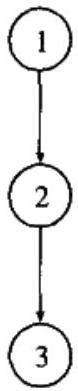
\includegraphics[width=\textwidth]{images/2025_05_15_6a28331d5e7c993ad07ag-034.jpg}
\end{center}

而对这同一串论证的分析,解析法尽管显得不够简洁,但更完整:

\begin{enumerate}
  \item 一个人种身上的线粒体变种越多,其进化史就越长;
  \item 出现在非洲人种身上的线粒体变种最多,\\
  因此非洲人种进化史最长。
\end{enumerate}

\begin{enumerate}
  \item 非洲人种进化史最长,
  \item 现代人类可能起源于进化史最长的人种,\\
  因此现代人类可能起源于非洲人种。
\end{enumerate}

这样的复合论证表明,一个孤立表达的命题既非前提也非结论。在一个论证中,作为假定出现的命题就是前提,被断定为从假定命题推出的命题就是结论。也就是说,"\logicterm{前提}"和"\logicterm{结论}"都是相对的(relative)术语。

\subsection{交织式论证}

几个论证复合在一起,语言表达上可能不是以串联的方式出现,而是以独特的方式相互交织,这就要求我们对它们做细致的分析。图示法特别适用于这种情况。例如,在约翰·洛克的名篇《政府论》中,下面一段话就有两个论证交织在一起:

\begin{quotation}
立法机构常年运作是不必要的,也是很不方便的;但行政机关常年运作是绝对必要的,因为不是总需要制定新的法律,但总需要执行已制定的法律。
\end{quotation}

上述论证的分支命题可以用数字表示为:(1)立法机构常年运作是不必要的,也是很不方便的,(2)行政机关常年运作是绝对必要的,(3)不是总需要制定新的法律,(4)总需要执行已制定的法律。将这段论证图示如下:

\begin{center}
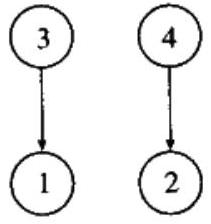
\includegraphics[width=\textwidth]{images/2025_05_15_6a28331d5e7c993ad07ag-035.jpg}
\end{center}

这个图示表明,第二个论证的结论出现在第一个论证的结论和前提之间,第一个论证的前提出现在第二个论证的结论和前提之间。这个图示还表明,两个结论都出现在它们的前提之前。

这个图示同样也展示了支持刑罚威慑理论的古罗马哲学家塞涅卡的两个相关论证的逻辑结构:
\begin{quotation}
(1)惩罚罪行不是因为罪行已经发生,(2)而是为了不发生新的罪行。[因为](3)过去的罪行不能被取消,(4)但是可以预防将来的罪行。
\end{quotation}

在这段话中,"惩罚罪行不是因为罪行已经发生"是其中一个论证的结论,其前提是"过去的罪行不能被取消"。"惩罚罪行是为了不发生新的罪行"是这段话中第二个论证的结论,其前提是"惩罚罪行可以预防将来的罪行"。

\chaptersummary{
论证分析是逻辑学的核心技能,主要包括\logicemph{解析法}和\logicemph{图示法}两种方法。\logicterm{解析法}通过重新组织和明确表述来揭示论证的逻辑结构,特别适合处理隐含前提和复杂的推理链。\logicterm{图示法}通过视觉化的方式直观展现前提与结论的支持关系,能够清晰地区分独立支持、联合支持等不同模式。

掌握这两种分析方法,能够帮助我们更准确地理解和评估各种论证,识别其逻辑结构的优势和缺陷,从而提高逻辑思维能力。在实际应用中,应根据论证的具体特点选择最适合的分析方法,或者将两种方法结合使用。
}